\documentclass{article}

\usepackage{a4wide}
\usepackage[utf8]{inputenc}
\usepackage[T1]{fontenc}
\usepackage[french]{babel}
\usepackage[babel=true]{csquotes} % guillemets français
\usepackage{graphicx}
\graphicspath{{Images/}}
\usepackage{color}
\usepackage{hyperref}
\hypersetup{colorlinks,linkcolor=,urlcolor=blue}

\usepackage{amsmath}
\usepackage{amssymb}


\title{UnivMap}
\author{Damien LAOUSSING, Dylan CHERRIER, L3 informatique}
\date{\today}

\begin{document}

\maketitle %% pour écrire le titre


%% Le résumé:
\begin{abstract}
  UnivMap est une application mobile iOS et Android destinée aux nouveaux
  étudiants afin de les aider à se repérer au sein de l'Université de la Réunion.
\end{abstract}


\section{Introduction}
\label{section:intro} % pour faire référence à la section ailleurs (\ref{...} voir plus bas)

Dans le cadre du projet de l'unité d'enseignement "Développement pour Mobiles", nous avons décidé de développer
une application iOS et Android. Cette application a pour but d'aider nos utilisateurs à se repérer à l'Université de la Réunion.

Le changement peut-être difficile pour certains étudiants réunionnais ou étranger.
Beaucoup de ces étudiants, découvrant leurs nouveau campus, sont souvent perdu pour trouver leur cours. Par conséquent,
ils arrivent généralement en retard et perdent ainsi leurs qualités d'apprentissages.
Aujourd'hui, afin de répondre au besoin de ces étudiants, nous allons vous présenter l'application UnivMap.

Dans un premier temps, nous verrons une description générale de l'application, puis nous analyserons
l'architecture du code. Ensuite, nous aborderons les difficultés rencontrés durant le développement
du projet pour enfin terminer par une conclusion.

\section{Description générale de l'application}


\begin{center}
    
\includegraphics[width=45mm, scale=0.5]{UnivMap-logo500x500.png}
\end{center}


L'application possède trois onglets : la carte de l'université, le calendrier des cours ainsi que des options.
La carte intègre des fonctionnalités permettant l'affichage des enseignements sous formes de cercle coloré, De plus,
des boutons sont à la disposition de l'utilisateur afin de les parcourir.
Le calendrier permet d'afficher sous forme d'une liste le planning de l'étudiant.
Les options inclus la possibilité de changer la langue et la couleur de l'arrière plan.

L'application utilise principalement la carte de l'API \textit{Mapbox}~\cite{mapboxDoc} développé par l'entreprise
du même nom sur les bases du logiciel libre et sur les données d'\textit{OpenStreetMap}~\cite{openstreetmapDoc}.
La persistance de donnée de notre application est gérer par le système interne, mais aussi par la plateforme
de Google, \textit{Firebase}~\cite{firebaseDoc}.



\newpage %% Passer a une autre page



\subsection{Présentation de la carte et annoations des points}

Tout d'abord, UnivMap requiert une connexion internet afin de géolocaliser son utilisateur mais aussi
pour récupérer des données indispensables à son fonctionnement (carte, liste des cours, ect...). Au lancement,
l'utilisateur se retrouve sur l'onglet de la carte avec toutes les positions des cours. En cliquant sur l'un d'eux,
un pop-up apparaît affichant les informations du cours (nom du cours, nom de l'enseignant, salle et horaire).\\

\begin{itemize}
    \item Point bleu : les marqueurs de couleur bleu représente la position des cours qui n'ont pas encore commencé.

    \item Point orange : le marqueur de couleur orange représente la position du cours qui commencera dans
    moins de deux heures.

    \item Point rouge : le marqueur de couleur rouge représente la position du cours qui a déjà débuté.

    \item Point gris : le marqueur de couleur gris représente la position des cours terminé.
\end{itemize}

\vspace{10pt}   %espace

\begin{center}
    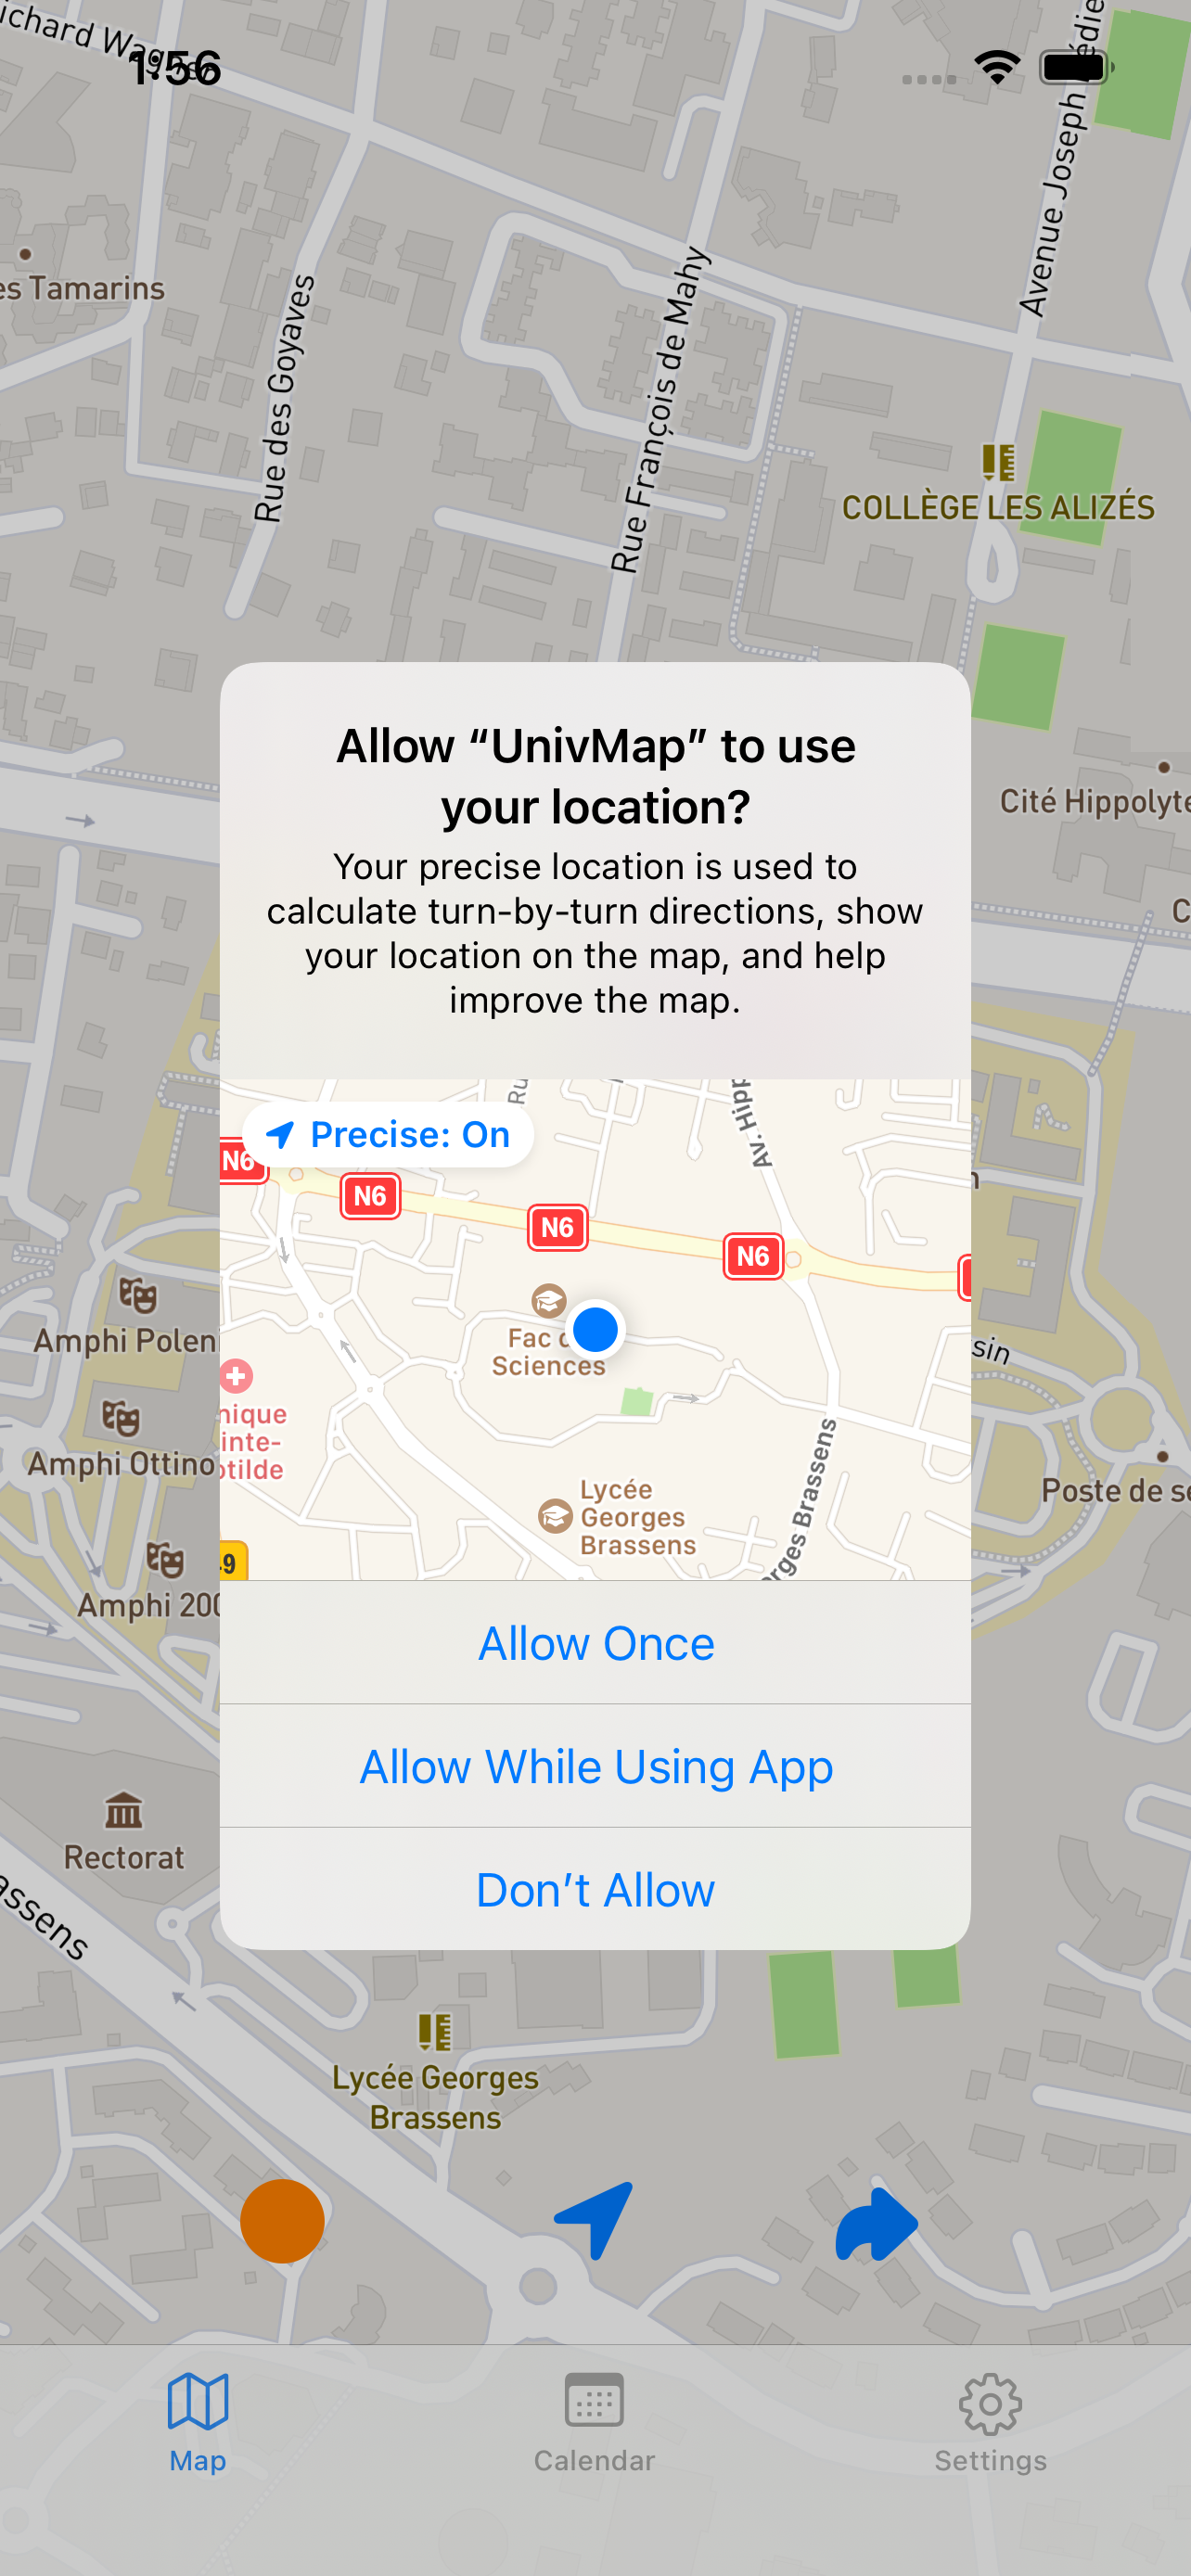
\includegraphics[width=45mm, scale=0.5]{allowUserLocation.png}
    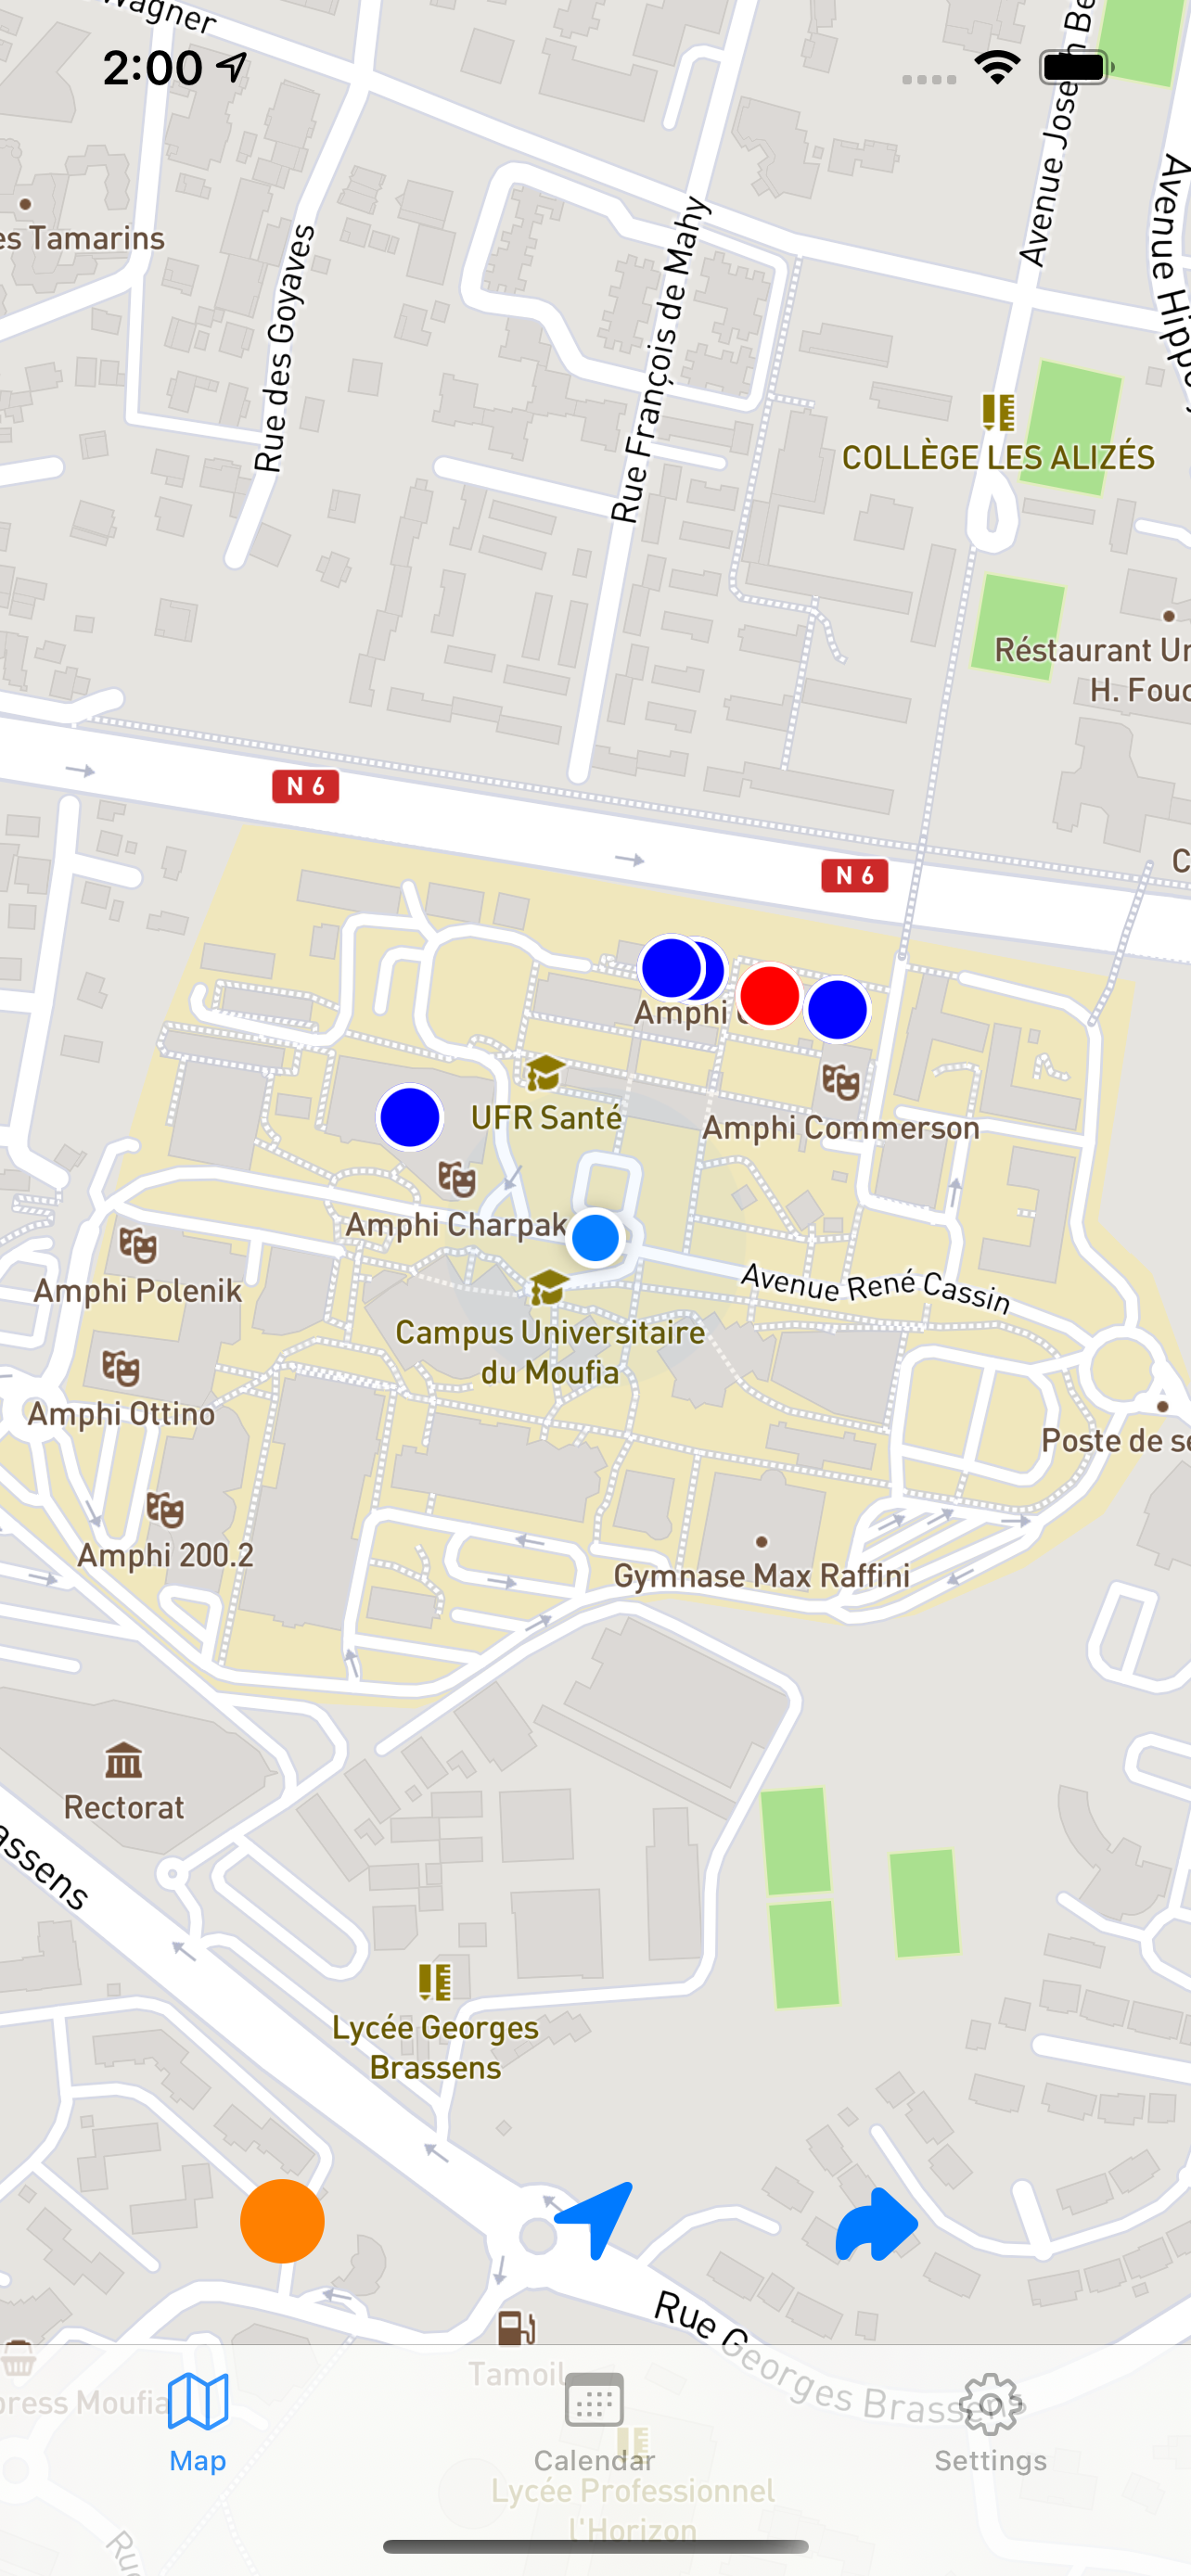
\includegraphics[width=45mm, scale=0.5]{map.png}
    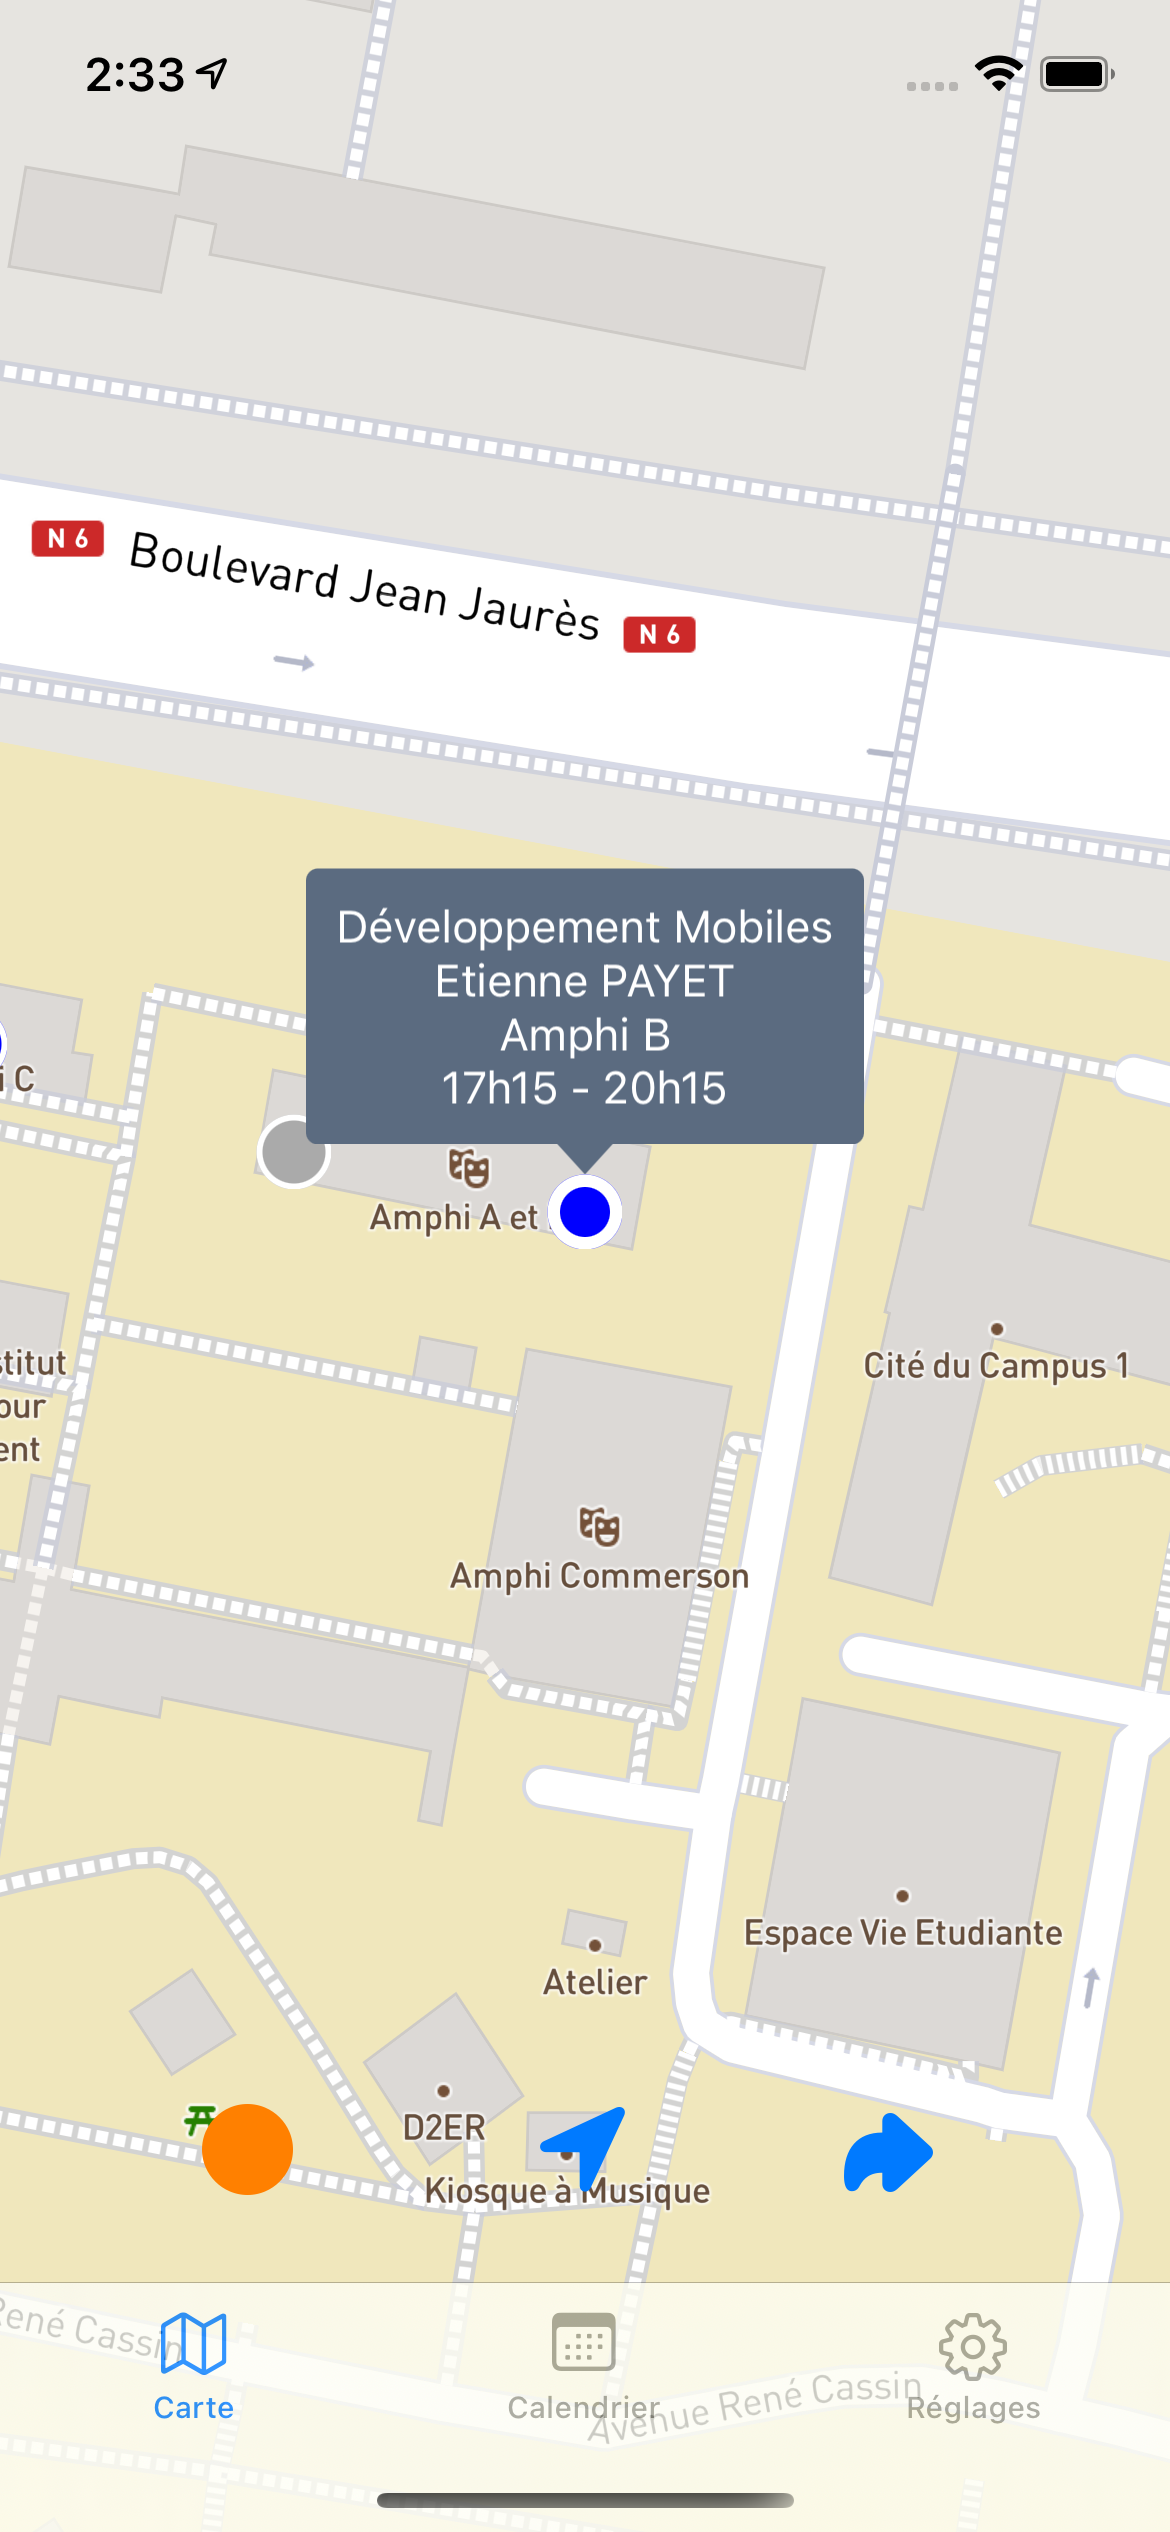
\includegraphics[width=45mm, scale=0.5]{point_bleu.png}
\end{center}

Les trois boutons du bas permettent de changer la vue de la caméra :\\

\begin{itemize}
    \item Bouton de gauche : parcourir les cours qui débuterons prochainement.

    \item Bouton du milieu : centrer sur la position de l'utilisateur.

    \item Bouton de droite : parcourir parmis chaque cours.
\end{itemize}



\newpage %% Passer a une autre page



\subsection{Calendrier : la liste des cours}

L'onglet calendrier permet l'affichage de tous les cours trier par ordre croissant selon l'heure. Pour récupérer ces
données, l'application utilise \textit{Firebase}~\cite{firebaseDoc}, un service d'hébergement en NoSQL
développer par Google. En sélectionnant le cours, l'application nous redirige vers une nouvelle vue,
affichant la position exacte de celui-ci.

\vspace{10pt}   %espace

\begin{center}
    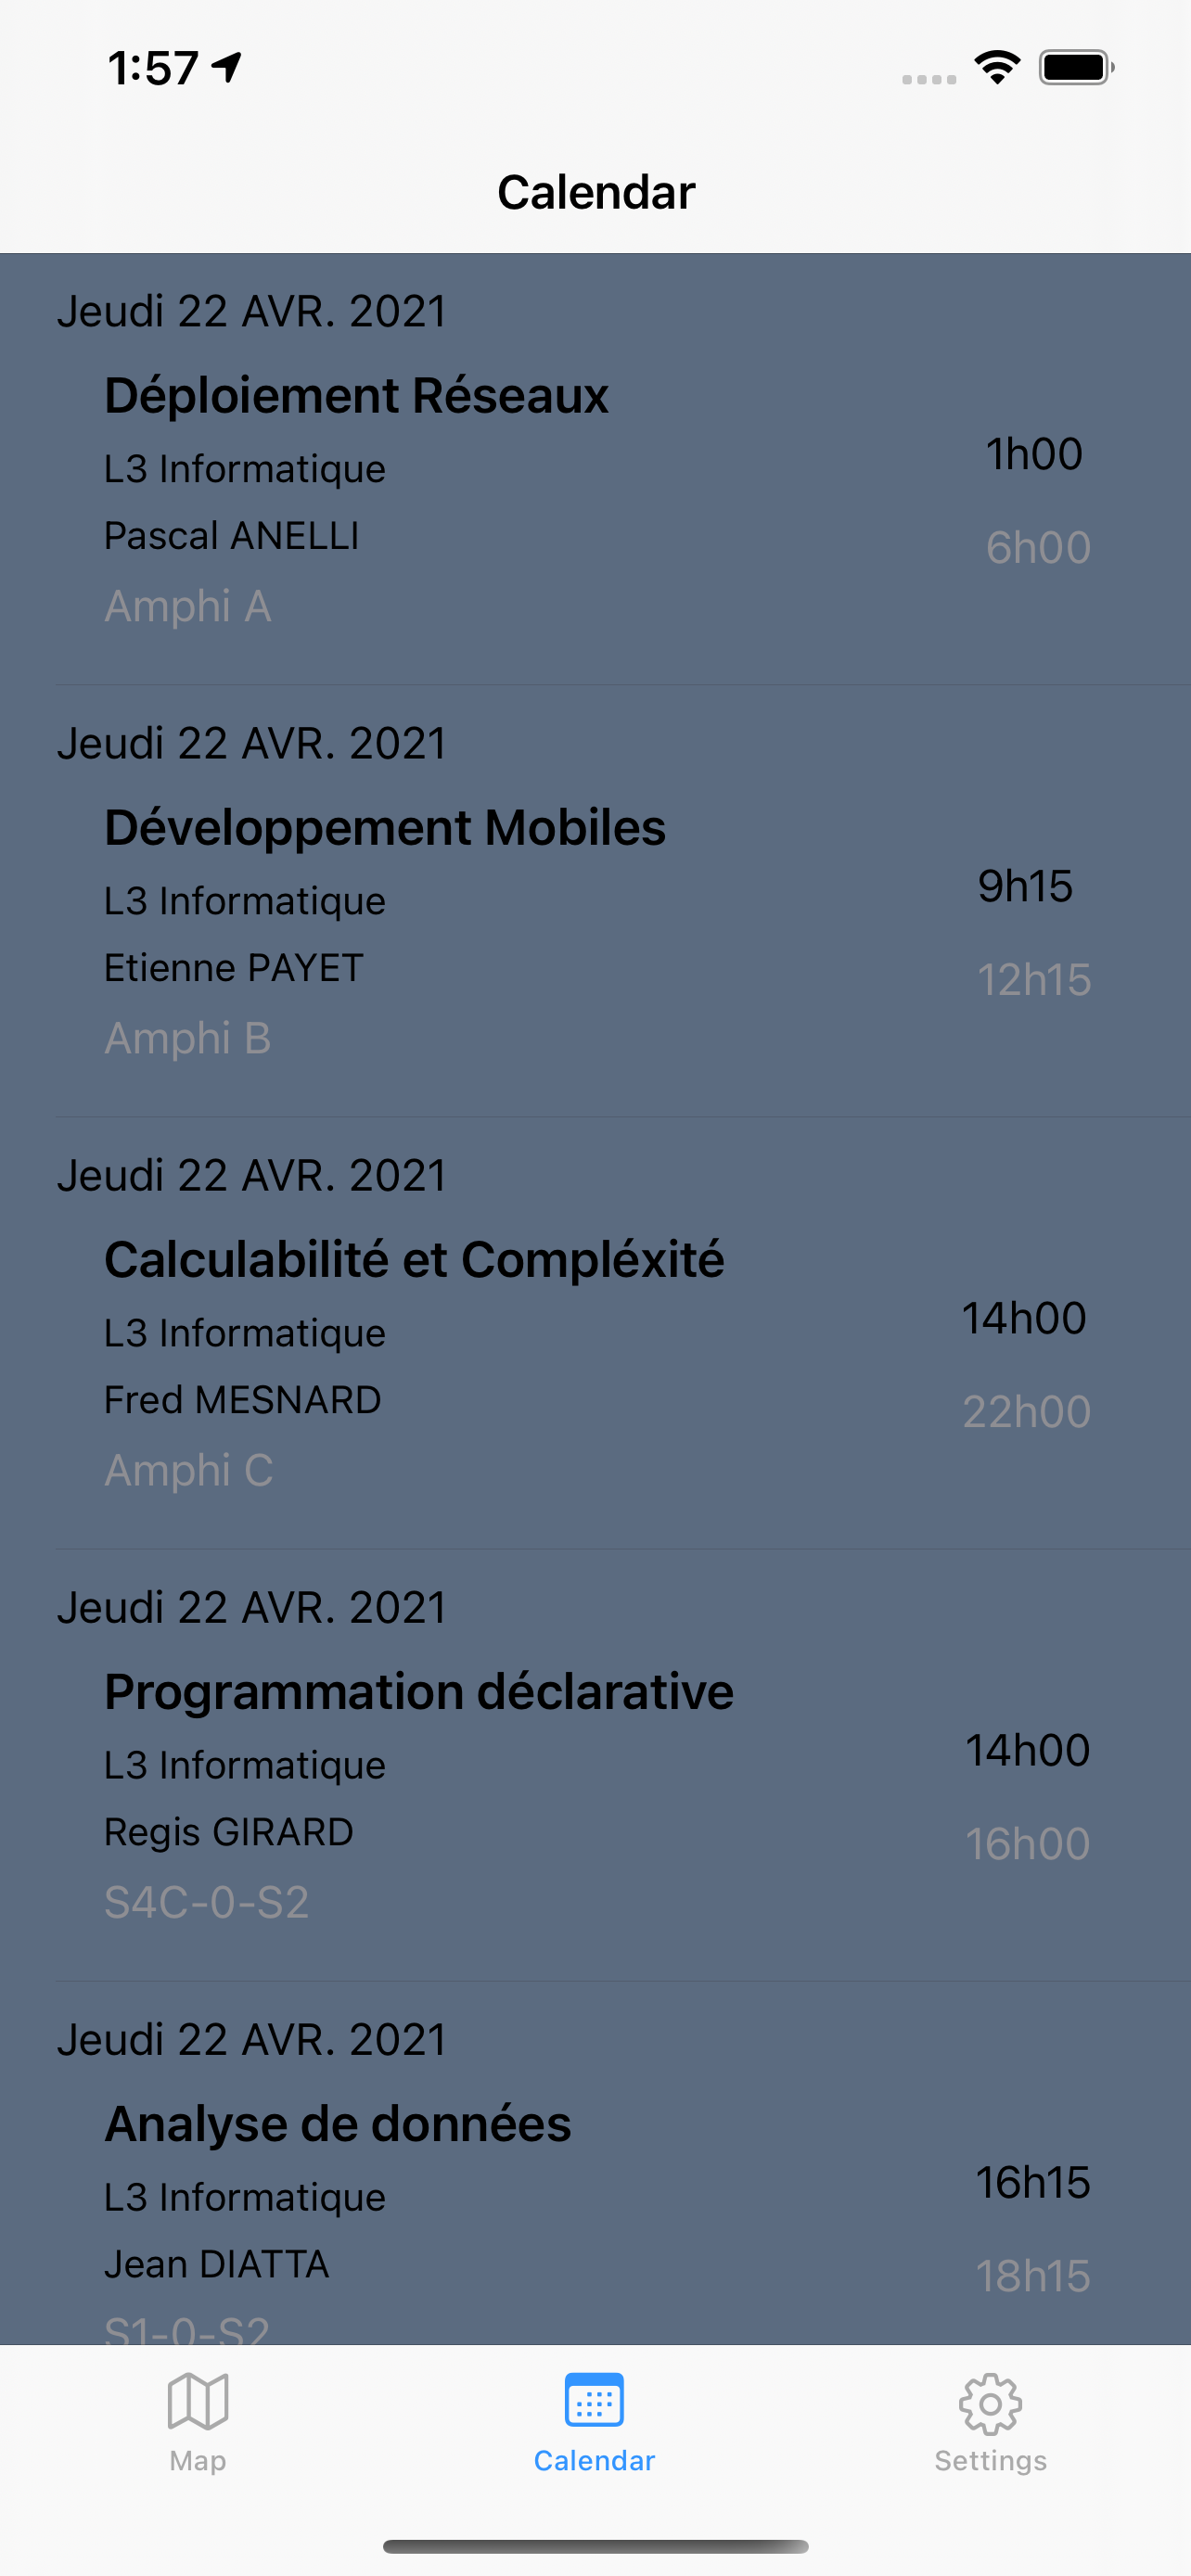
\includegraphics[width=50mm, scale=0.5]{calendar.png}
    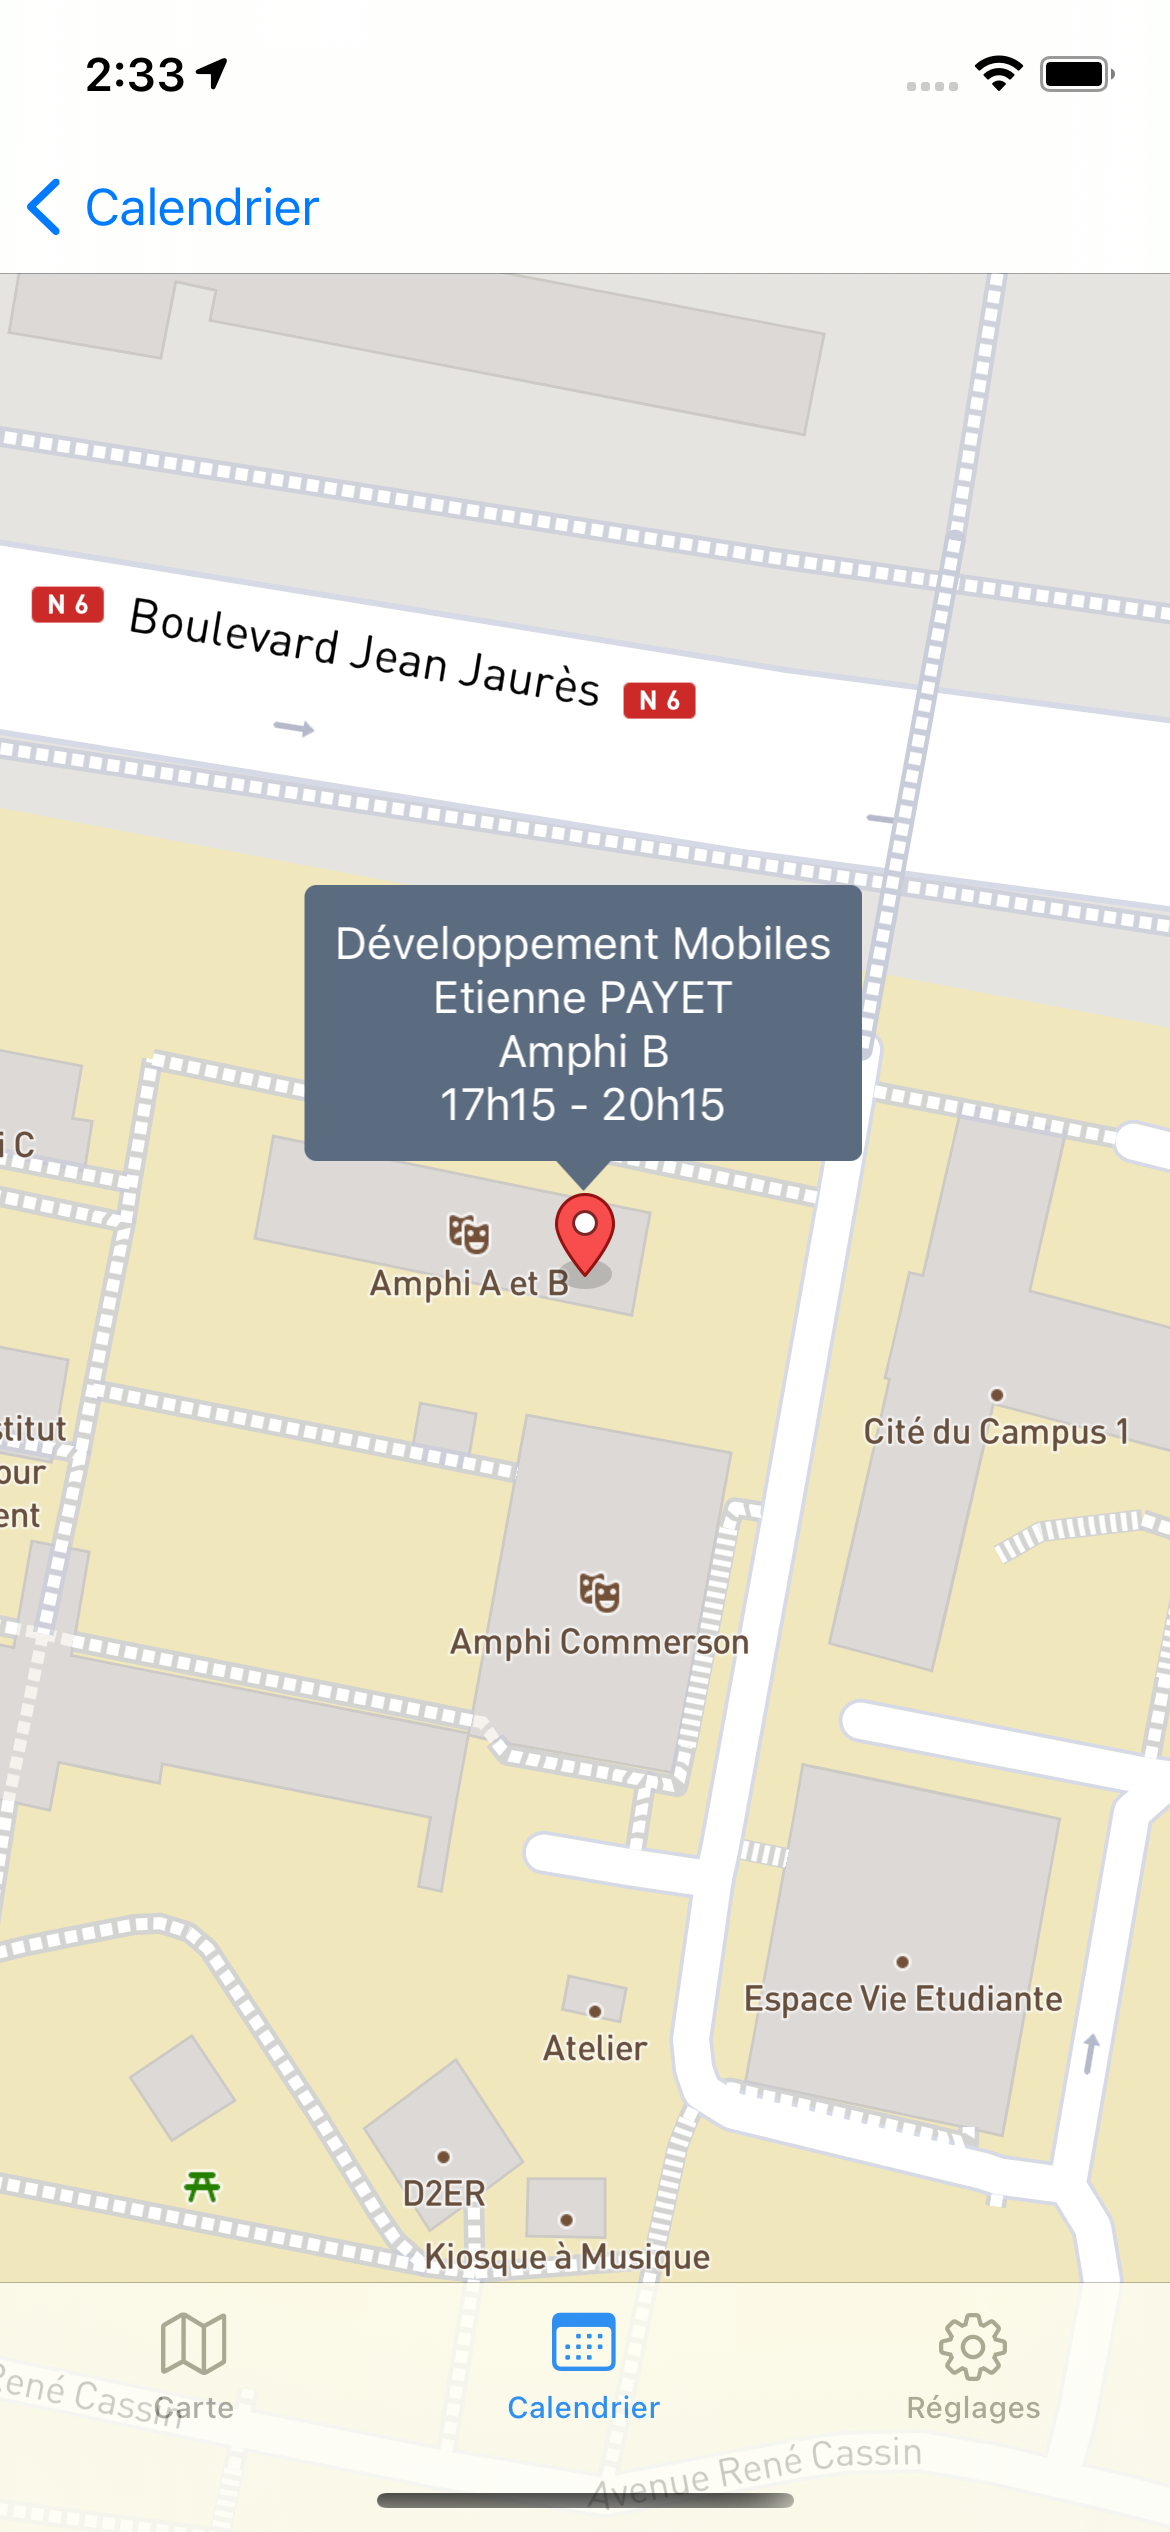
\includegraphics[width=50mm, scale=0.5]{calendar_position.png}
\end{center}



\newpage %% Passer a une autre page



\subsection{Présentation des paramétrages}
Enfin l'onglet des paramètres de l'application, présenté sous forme de liste (générer dynamiquement), permet à l'utilisateur
de mieux s'approprier l'application et d'en apprendre d'avantage. À travers cet onglet, nous voulions encore une fois
mettre en valeur notre volonté d'aider les étudiants, tout en leur apportant le maximum de confort. Pour cela, nous avons
choisi de mettre en avant, pour cette première version d'UnivMap, les paramètres suivants :\\

\begin{itemize}
    \item Le choix de la langue : la possibilité de choisir la langue de l'application est une option, qui nous semblent toujours indispensable.
    Cette option augmente le confort certe, mais surtout permet au public de différentes nationalités de l'utiliser.
    Pour cette option, l'utilisateur a le choix entre utiliser la même langue que son appareil, ou utiliser une des langues listées ci-dessous.   

    \item Le choix du thème de l'application : le choix du thème de l'application permet à l'utilisateur de choisir la couleur de fonds.
    
    \item L'assistance : en cas de problème, l'utilisateur est invité à contacter l'assistance par mail. Ainsi en cliquant sur "assistance",
    puis envoyer, il est redirigé vers une application de mail. 
    
    \item Mais aussi les mentions légales et la confidentialité : ces deux options sont présent à titre informatif et sont indispensables à tout
    application. Ces deux parties doivent faire apparaître respectivement la charte de protection des données personnelles,
    ainsi que les CGU(conditions générales d'utilisation), etc...
    
    \item Et enfin, UnivMap : cette option est présente pour permettre à l'utilisateur d'en apprendre d'avantage sur UnivMap. Notamment,
    le but de l'application ainsi que les développeurs ayant contribué à sa création.
    
\end{itemize}

\vspace{10pt}   %espace

\begin{center}
    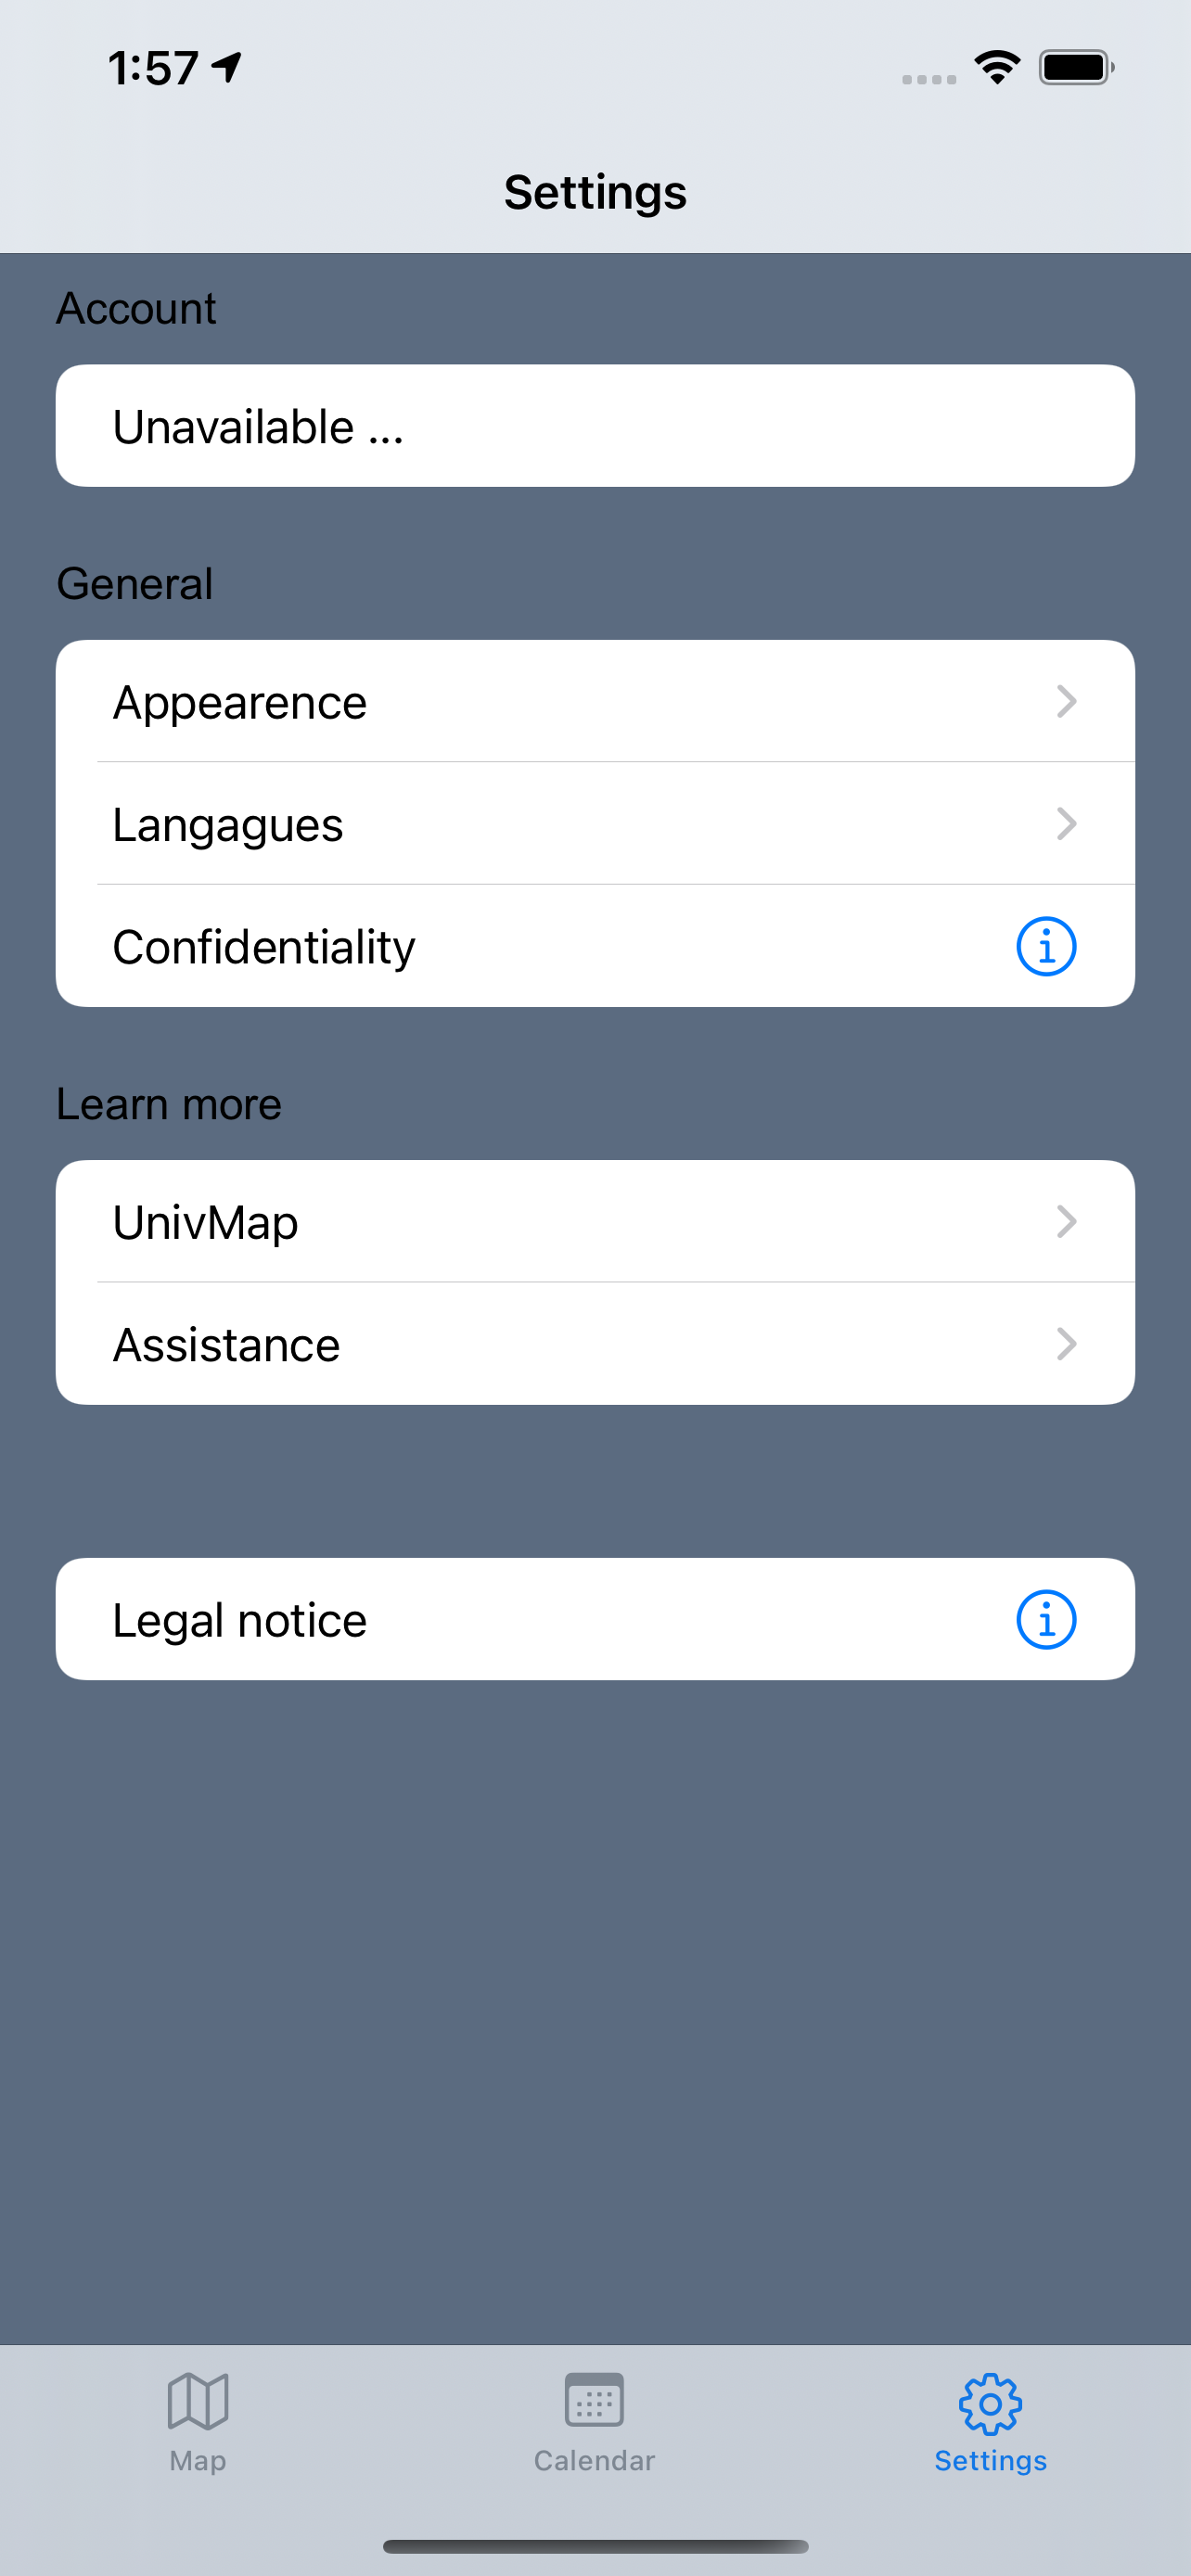
\includegraphics[width=35mm, scale=0.5]{setting.png}
    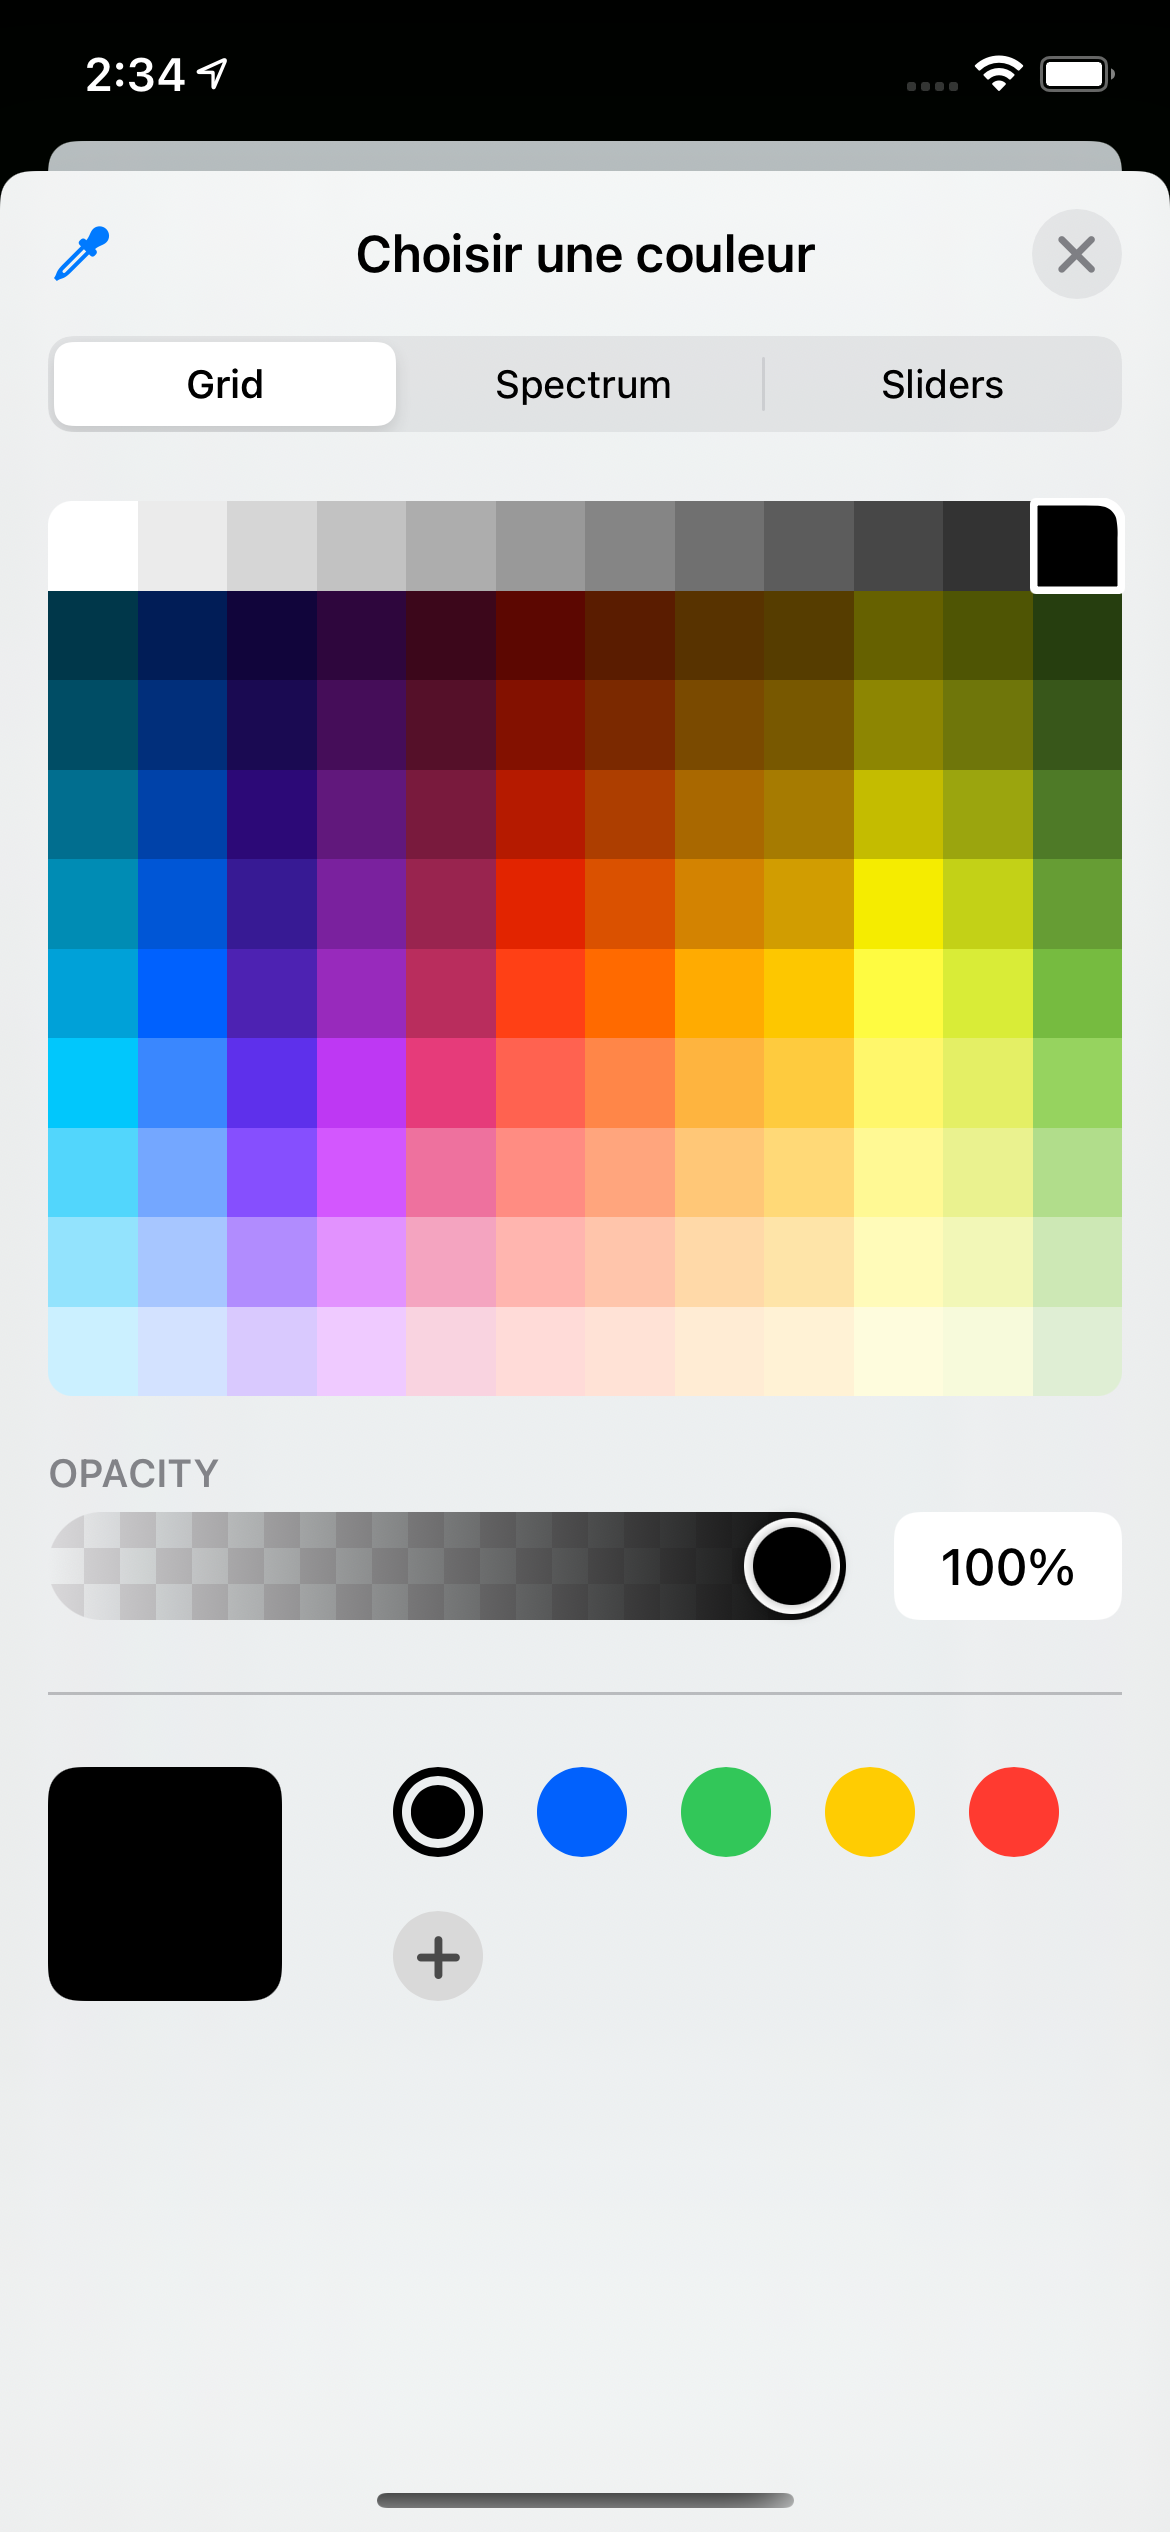
\includegraphics[width=35mm, scale=0.5]{setting_appearance.png}
    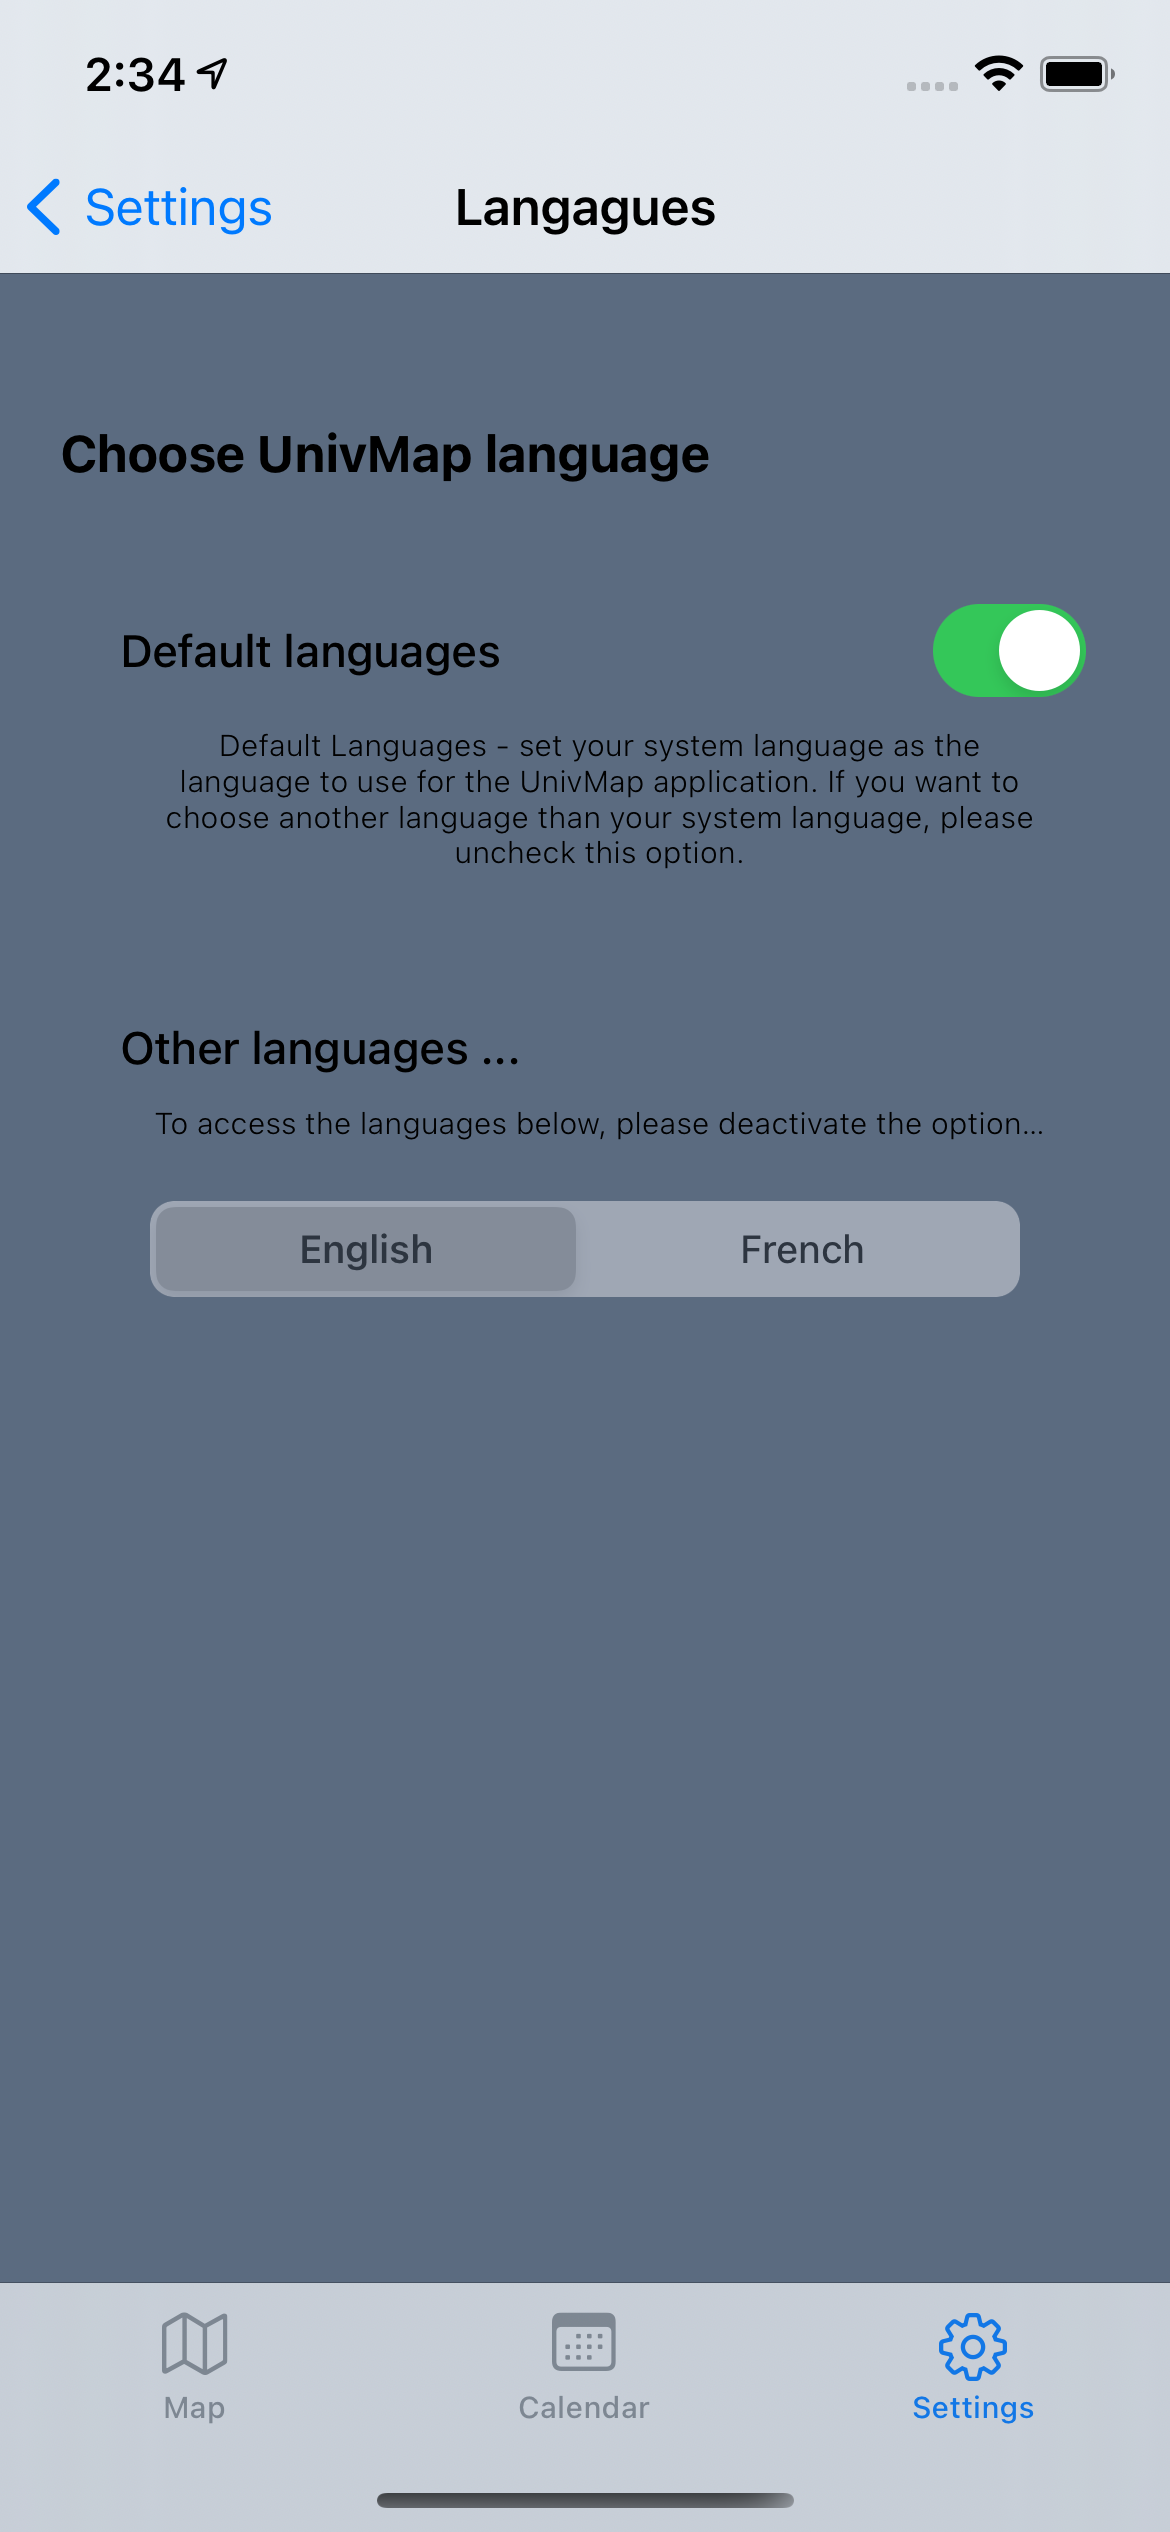
\includegraphics[width=35mm, scale=0.5]{setting_languageOn.png}
    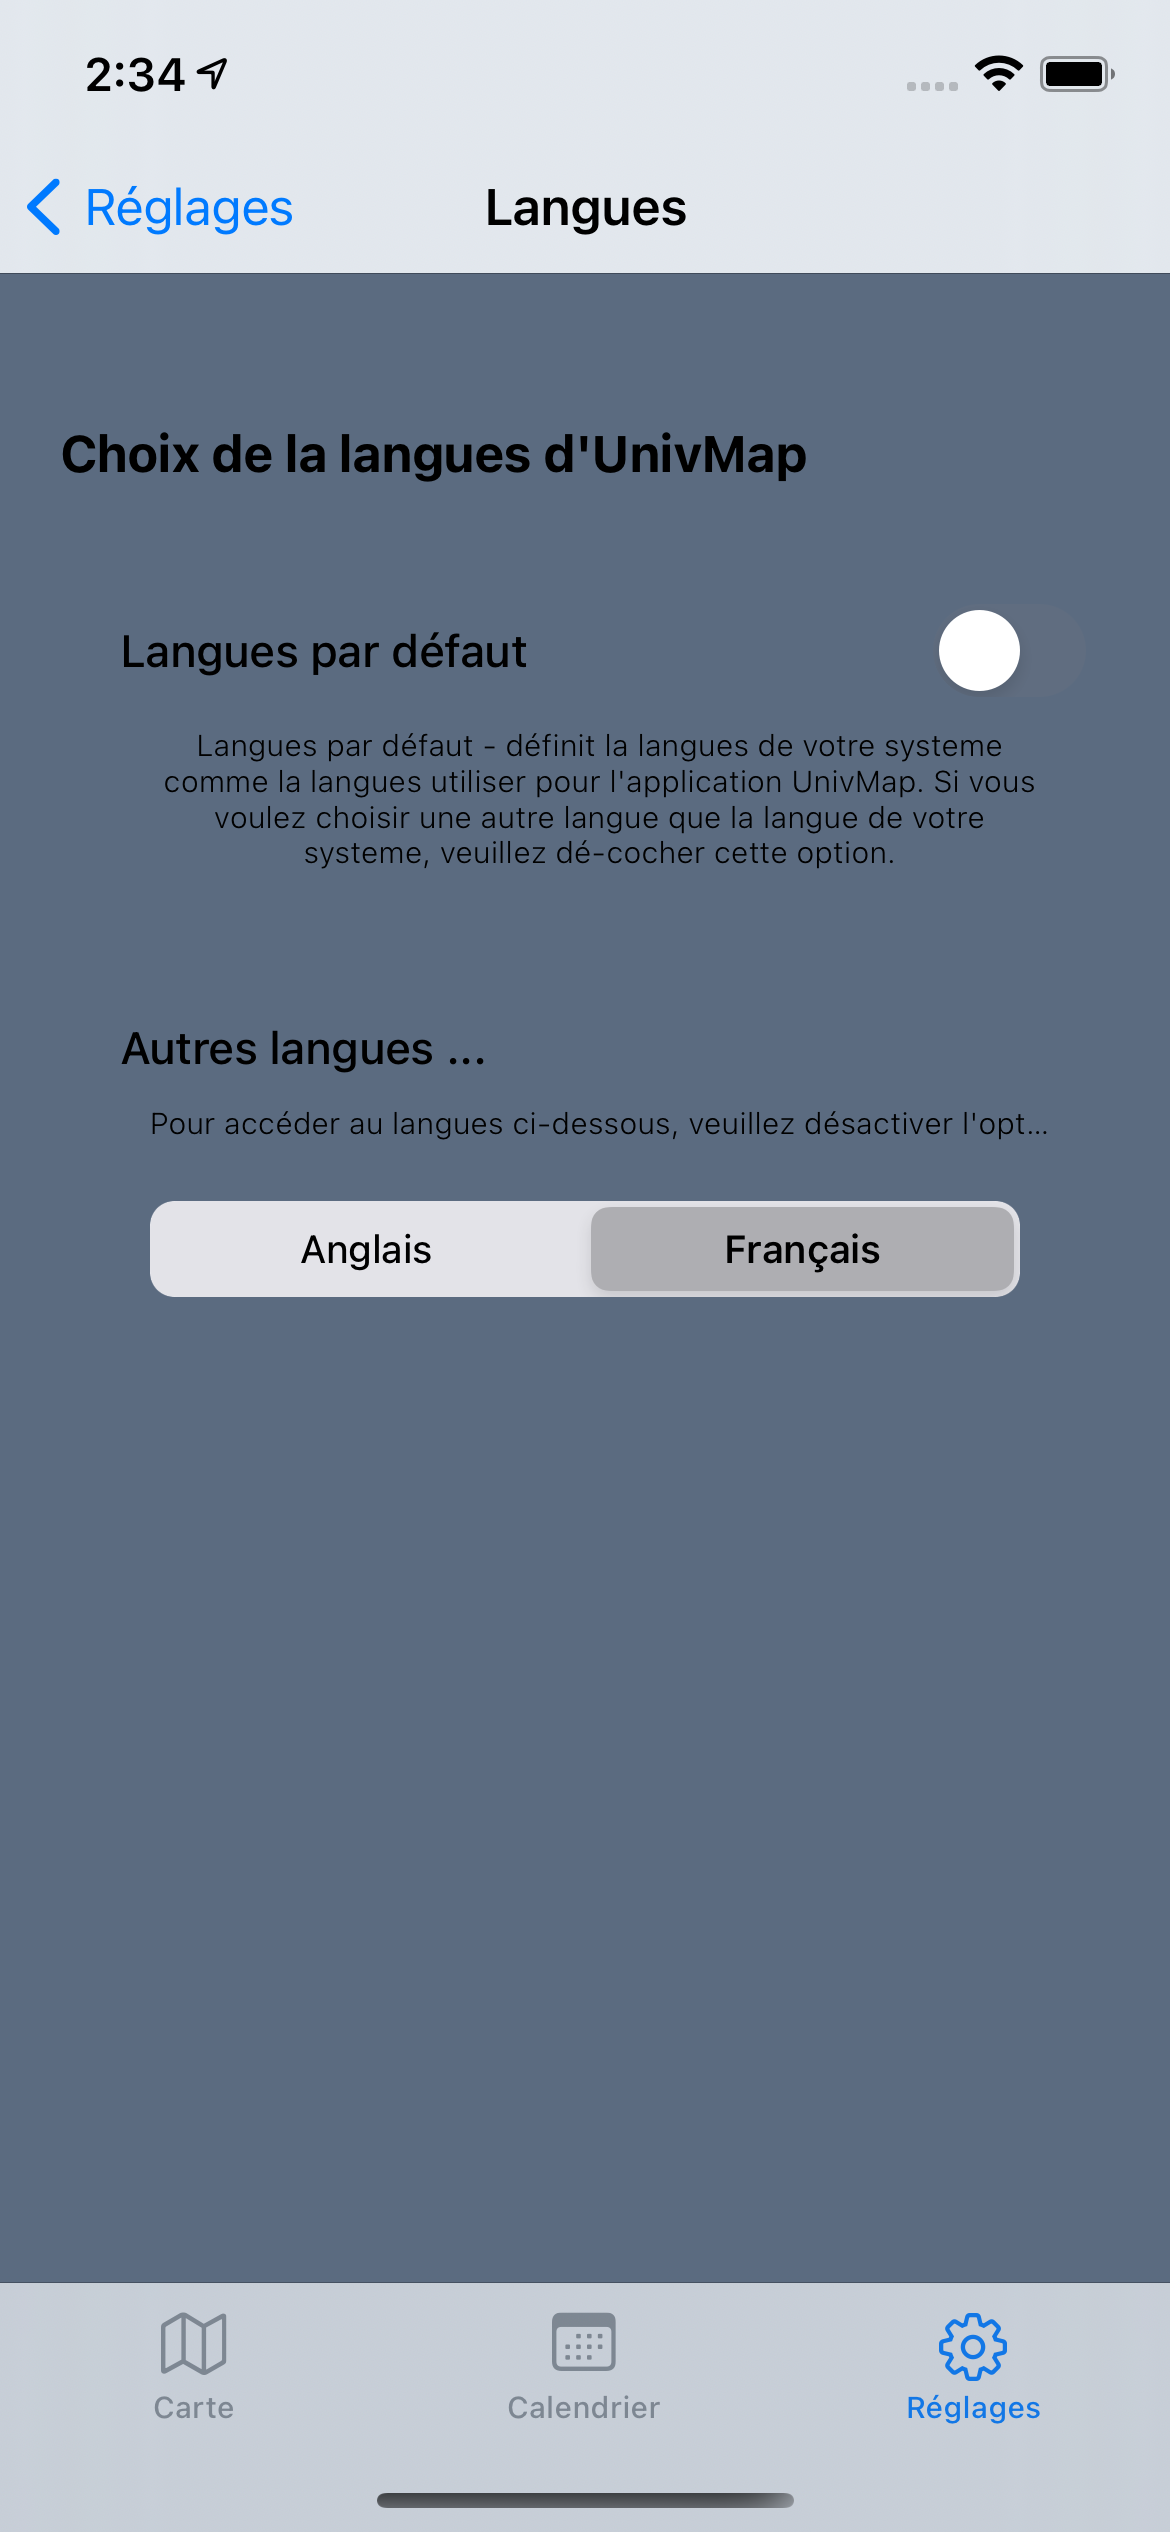
\includegraphics[width=35mm, scale=0.5]{setting_languageOff.png}
\end{center}



\newpage %% Passer a une autre page



\section{Architecture du code}
% \ref{...} permet de faire référence à un élément défini
% ailleurs dans le document (voir \label{...} plus haut).
UnivMap est une application iOS et Android développer respectivement en Swift et Java.


\subsection{Android} %% une sous-section
\label{subsection:Android} 


\subsubsection{Java : Ouverture à la base de donnée}
\label{subsubsection:Java : Ouverture à la base de donnée} 
Cette fonction permet d'ouvrir la connexion à Firebase et de récupérer les données selon la clé. Elle retourne
une liste d'objet en Callback.

\begin{verbatim}
    public void getAllData(ListPlanningCallback listPlanningCallback) {
        db.collection("planning")
                .get()
                .addOnCompleteListener(new OnCompleteListener<QuerySnapshot>() {
                    @Override
                    public void onComplete(@NonNull Task<QuerySnapshot> task) {
                        if (task.isSuccessful()) {
                            List<Planning> listLocal = new ArrayList<Planning>();

                            for (QueryDocumentSnapshot document : task.getResult()) {
                                //Log.d(TAG, document.getId() + " => " + document.getData());

                                String nom = document.getString("nom");
                                String filiere = document.getString("filiere");
                                String enseignant = document.getString("enseignant");
                                String hDebut = document.getString("hDebut");
                                String hFin = document.getString("hFin");
                                String mDebut = document.getString("mDebut");
                                String mFin = document.getString("mFin");
                                String salle = document.getString("salle");
                                String latitude = document.getString("latitude");
                                String longitude = document.getString("longitude");

                                Planning planning = new Planning(nom, filiere, enseignant,
                                hDebut, hFin, mDebut, mFin, salle, latitude, longitude);

                                listLocal.add(planning);

                            }
                            listPlanningCallback.onCallback(listLocal);
                        } else {
                            Log.d(TAG, "Error getting documents: ", task.getException());
                        }
                    }
                });

    }
\end{verbatim}




\newpage %% Passer a une autre page




\subsubsection{Java : Choix de la langue}
La première fonction permet de modifier la langue d'une chaîne de caractère et la seconde permet de récupérer la langue de l'appareil :

\begin{verbatim}
   
    public static void setLocale(Activity activity, String languageCode) {
        Locale locale = new Locale(languageCode);
        Locale.setDefault(locale);
        Resources resources = activity.getResources();
        Configuration config = resources.getConfiguration();
        
        if (Build.VERSION.SDK_INT >= Build.VERSION_CODES.JELLY_BEAN_MR1) {
            config.setLocale(locale);
        } else {
            config.locale = locale;
        }
        resources.updateConfiguration(config, resources.getDisplayMetrics());

    }

    public static String currentLanguage(){
        return Resources.getSystem().getConfiguration().locale.getLanguage();
    }

\end{verbatim}




\newpage %% Passer a une autre page




\subsection{iOS} %% une autre sous-section
\label{subsection:iOS} 


\subsubsection{Swift : Ouverture à la base de donnée}
\label{subsubsection:Swift : Ouverture à la base de donnée} 
Contrairement à la section~\ref{subsubsection:Java : Ouverture à la base de donnée}. Le code en Swift permettant de récupérer les données
est facilité. Il n'y a aucunement besoin d'une fonction Callback pour ajouter à une liste d'objet.

\begin{verbatim}
    db.collection("planning").getDocuments() { [self] (querySnapshot, err) in
    if let err = err {
        print("Error getting documents: \(err)")
    } else {
        
        for document in querySnapshot!.documents {
            if let nom = document.data()["nom"] as? String,         //recup data selon clé
                let filiere = document.data()["filiere"] as? String,
                let enseignant = document.data()["enseignant"] as? String,
                let hDebut = document.data()["hDebut"] as? String,
                let hFin = document.data()["hFin"] as? String,
                let mDebut = document.data()["mDebut"] as? String,
                let mFin = document.data()["mFin"] as? String,
                let salle = document.data()["salle"] as? String,
                let latitude = document.data()["latitude"] as? String,
                let longitude = document.data()["longitude"] as? String{
            
                self.listPlanning.append(Planning(nom: nom, filiere: filiere,
                enseignant: enseignant, hDebut: hDebut, hFin: hFin, mDebut: mDebut, mFin: mFin,
                salle: salle, latitude: latitude, longitude: longitude ))
                

                (...)
            }
            (...)
            
        }   
    }


\end{verbatim}




\newpage %% Passer a une autre page




\subsubsection{Swift : Choix de la langue}
Cette fonction permet la traduction d'une chaîne de caractère de trois manières différentes :

\begin{itemize}
    \item Selon la langue passé en paramètre : affiche toujours un texte dans une langue en particulier ! 

    \item Selon la langue par défaut : affiche toujours un texte dans la langue par défaut, c'est-à-dire la langue de l'appareil.

    \item Selon le choix de l'utilisateur : affiche le texte dans la langue choisi par l'utilisateur.
\end{itemize}

\begin{verbatim}
    extension String {
    func localized(str:String?) -> String{
        if let language = str{
            let path = Bundle.main.path(forResource: language, ofType: "lproj")
            let bundle = Bundle(path: path!)
            return NSLocalizedString(self, tableName: "Localizable", bundle: bundle!,
            value: self, comment: "nil")
        }
        if(UserDefaults.standard.bool(forKey: "switchState")){
            return NSLocalizedString(self, tableName: "Localizable", bundle: .main,
            value: self, comment: "nil")
        }
        let path = Bundle.main.path(forResource: UserDefaults.standard.string(forKey: "language"), 
        ofType: "lproj")
        let bundle = Bundle(path: path!)
        return NSLocalizedString(self, tableName: "Localizable", bundle: bundle!, value: self,
        comment: "nil")
    }
}  
\end{verbatim}


\newpage %% Passer a une autre page


\section{Quelques points délicats/intéressants}

Durant le développement de notre application, nous avons rencontrés des difficultés concernant la prise en main
de nouveaux outils de travail tels que Git.
De plus, l'implémentation de l'API Mapbox et de \textit{Firebase}~\cite{firebaseDoc} a beaucoup ralenti
le développement sur iOS. En effet, \textit{Firebase}~\cite{firebaseDoc} étant développer par Google, son importation
était une épreuve sur Xcode. Afin d'installer les dépendances requises sur iOS, nous avons utilisés
le gestionnaire de dépendances \textit{CocoaPods}~\cite{cocoapodsDoc}.
Malgré toutes ces difficultés, l'API Mapbox nous a permis de finir ce projet dans les temps.
Mapbox étant très complet, possèdent ses propres classes et fonctions permettant aux développeurs de l'intégrer facilement dans leurs projets.
Concernant \textit{Firebase}~\cite{firebaseDoc}, son utilisation est plus aisé en Swift. En effet, Swift permet
l'ajout de valeur dans une liste d'objet déclarer globalement. Contrairement à Java, ou il a fallu passé par une
fonction callback (voir section~\ref{subsubsection:Java : Ouverture à la base de donnée}) pour récupérer les données.

La traduction de l'application, en iOS, révèle la puissance des extensions permettant ainsi de rajouter des fonctions, structures, etc...
Et cela même à des classes normalement inaccessibles (code source du langage de programmation) comme la classe String. Néanmoins, il était plus simple de gérer la traduction en Java.
La gestion de la traduction et de l'apparence de l'application, nous a confronté au cycle de vie (des view/activity) des différentes plateformes.
Et l'utilisation des données persistances sous forme de couple (clé, valeur), pour enregistrer des petites données (préférences utilisateurs), est remarquable.
Les données persistantes nous ont même permis de récupérer des paramètres initiales et exécuter du code (la première fois qu'on lance l'application).


\subsection{UnivMap 2.0 à suivre}
À la fin du développement de notre application,  bien qu'elle soit fonctionnelle, certaines améliorations sont à venir, telles que l'ajout :
\begin{itemize}
    \item du choix du planning selon la fillière;

    \item de notification lorsque l'emploi du temps est modifié;

    \item d'un onglet accueil avec des redirections vers d'autres plateformes de l'Université et l'affichages d'évèments;
    
    \item de filtre sur la carte.
    
\end{itemize}



\section{Conclusion}


Enfin pour conclure le rapport, ce projet nous a beaucoup apporté en tant que développeur mobile
que ce soit sur les connaissances basiques en passant par l'implémentation d'API. Le développement d'UnivMap
à montré que le travail de groupe, l'entraide et la communication étaient primordial.
Malgré quelque appréhension face à l'idée de l'application, notre binôme à su montré son ambition et
sa persévérance d'atteindre l'objectif d'aider de nouveaux étudiants.


%% - travail de groupe
%% - l'implémentation d'API
%% - solidifier nos connaissances en tant que développeur mobiles



%%% La bibliographie:
\bibliographystyle{plain}
\bibliography{ma_biblio}

\end{document}



